\documentclass {article}
\usepackage{graphicx}
\DeclareGraphicsExtensions{.pdf,.png,.jpg}% No es necesario
\usepackage{float}
\usepackage{subfigure}
% indicar extensión.
\begin{document} % Compilar PDFLaTeX
\begin{figure}[h!]
	\centering
	\subfigure[Converge]{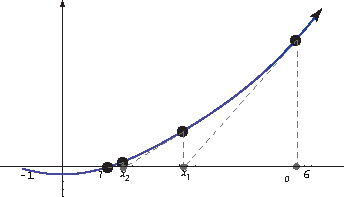
\includegraphics[scale=0.5]{images/newton6}}
	\subfigure[Diverge]{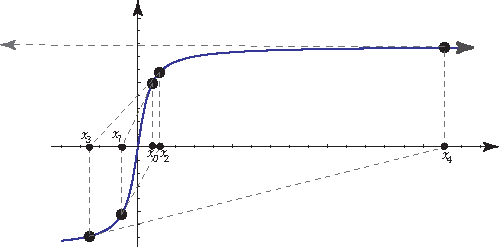
\includegraphics[scale=0.5]{images/newton5}}
	\subfigure[Ciclo]{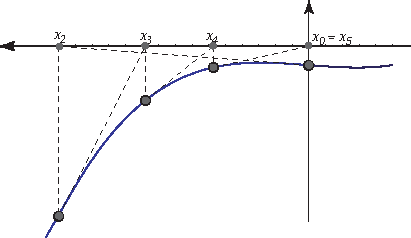
\includegraphics[scale=0.5]{images/newton4}}
	\caption{Iteración de Newton}
\end{figure}
\end{document}